\section{Injury and Death}
Your hit points measure how hard you are to kill. No matter how many hit points you lose, your character isn't hindered in any way until your hit points drop to 0 or lower.

\subsection{Loss Of Hit Points}
The most common way that your character gets hurt is to take lethal damage and lose hit points.

\textbf{What Hit Points Represent:} Hit points mean two things in the game world: the ability to take physical punishment and keep going, and the ability to turn a serious blow into a less serious one.

\textbf{Effects of Hit Point Damage:} Damage doesn't slow you down until your current hit points reach 0 or lower. At 0 hit points, you're disabled.

At from $-1$ to $-9$ hit points, you're dying.

At $-10$ or lower, you're dead.

\textbf{Massive Damage:} If you ever sustain a single attack deals 50 points of damage or more and it doesn't kill you outright, you must make a DC 15 Fortitude save. If this saving throw fails, you die regardless of your current hit points. If you take 50 points of damage or more from multiple attacks, no one of which dealt 50 or more points of damage itself, the massive damage rule does not apply.

\subsection{Disabled (0 Hit Points)}
When your current hit points drop to exactly 0, you're disabled.

You can only take a single move or standard action each turn (but not both, nor can you take full-round actions). You can take move actions without further injuring yourself, but if you perform any standard action (or any other strenuous action) you take 1 point of damage after the completing the act. Unless your activity increased your hit points, you are now at $-1$ hit points, and you're dying.

Healing that raises your hit points above 0 makes you fully functional again, just as if you'd never been reduced to 0 or fewer hit points.

You can also become disabled when recovering from dying. In this case, it's a step toward recovery, and you can have fewer than 0 hit points (see Stable Characters and Recovery, below).

\subsection{Dying ($-1$ to $-9$ Hit Points)}
When your character's current hit points drop to between $-1$ and $-9$ inclusive, he's dying.

A dying character immediately falls unconscious and can take no actions.

A dying character loses 1 hit point every round. This continues until the character dies or becomes stable (see below).

\subsection{Dead ($-10$ Hit Points or Lower)}
When your character's current hit points drop to $-10$ or lower, or if he takes massive damage (see above), he's dead. A character can also die from taking ability damage or suffering an ability drain that reduces his Constitution to 0.

\begin{figure*}[b!]
\centering
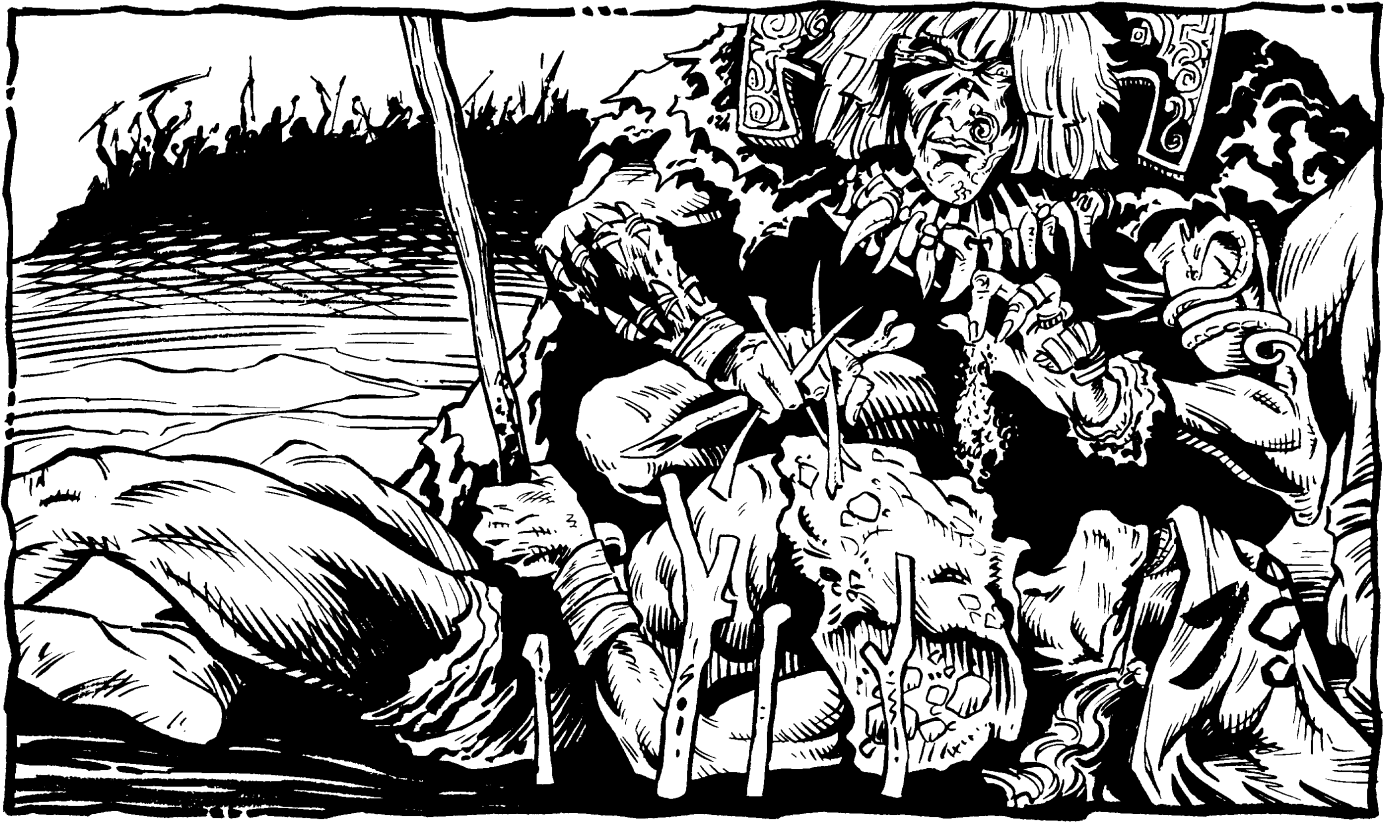
\includegraphics[width=\textwidth]{images/heal-1.png}
\WOTC
\end{figure*}
\subsection{Stable Characters and Recovery}
On the next turn after a character is reduced to between $-1$ and $-9$ hit points and on all subsequent turns, roll d\% to see whether the dying character becomes stable. He has a 10\% chance of becoming stable. If he doesn't, he loses 1 hit point. (A character who's unconscious or dying can't use any special action that changes the initiative count on which his action occurs.)

If the character's hit points drop to $-10$ or lower, he's dead.

You can keep a dying character from losing any more hit points and make him stable with a DC 15 \skill{Heal} check.

If any sort of healing cures the dying character of even 1 point of damage, he stops losing hit points and becomes stable.

Healing that raises the dying character's hit points to 0 makes him conscious and disabled. Healing that raises his hit points to 1 or more makes him fully functional again, just as if he'd never been reduced to 0 or lower. A spellcaster retains the spellcasting capability she had before dropping below 0 hit points.

A stable character who has been tended by a healer or who has been magically healed eventually regains consciousness and recovers hit points naturally. If the character has no one to tend him, however, his life is still in danger, and he may yet slip away.

\textbf{Recovering with Help:} One hour after a tended, dying character becomes stable, roll d\%. He has a 10\% chance of becoming conscious, at which point he is disabled (as if he had 0 hit points). If he remains unconscious, he has the same chance to revive and become disabled every hour. Even if unconscious, he recovers hit points naturally. He is back to normal when his hit points rise to 1 or higher.

\textbf{Recovering without Help:} A severely wounded character left alone usually dies. He has a small chance, however, of recovering on his own.

A character who becomes stable on his own (by making the 10\% roll while dying) and who has no one to tend to him still loses hit points, just at a slower rate. He has a 10\% chance each hour of becoming conscious. Each time he misses his hourly roll to become conscious, he loses 1 hit point. He also does not recover hit points through natural healing.

Even once he becomes conscious and is disabled, an unaided character still does not recover hit points naturally. Instead, each day he has a 10\% chance to start recovering hit points naturally (starting with that day); otherwise, he loses 1 hit point.

Once an unaided character starts recovering hit points naturally, he is no longer in danger of naturally losing hit points (even if his current hit point total is negative).

\subsection{Healing}
After taking damage, you can recover hit points through natural healing or through magical healing. In any case, you can't regain hit points past your full normal hit point total.

\textbf{Natural Healing:} With a full night's rest (8 hours of sleep or more), you recover 1 hit point per character level. Any significant interruption during your rest prevents you from healing that night.

If you undergo complete bed rest for an entire day and night, you recover twice your character level in hit points.

\textbf{Magical Healing:} Various abilities and spells can restore hit points.

\textbf{Healing Limits:} You can never recover more hit points than you lost. Magical healing won't raise your current hit points higher than your full normal hit point total.

\textbf{Healing Ability Damage:} Ability damage is temporary, just as hit point damage is. Ability damage returns at the rate of 1 point per night of rest (8 hours) for each affected ability score. Complete bed rest restores 2 points per day (24 hours) for each affected ability score.

\subsection{Temporary Hit Points}
Certain effects give a character temporary hit points. When a character gains temporary hit points, note his current hit point total. When the temporary hit points go away the character's hit points drop to his current hit point total. If the character's hit points are below his current hit point total at that time, all the temporary hit points have already been lost and the character's hit point total does not drop further.

When temporary hit points are lost, they cannot be restored as real hit points can be, even by magic.

\textbf{Increases in Constitution Score and Current Hit Points:} An increase in a character's Constitution score, even a temporary one, can give her more hit points (an effective hit point increase), but these are not temporary hit points. They can be restored and they are not lost first as temporary hit points are.

\subsection{Nonlethal Damage}
\textbf{Dealing Nonlethal Damage:} Certain attacks deal nonlethal damage. Other effects, such as heat or being exhausted, also deal nonlethal damage. When you take nonlethal damage, keep a running total of how much you've accumulated. Do not deduct the nonlethal damage number from your current hit points. It is not "real" damage. Instead, when your nonlethal damage equals your current hit points, you're staggered, and when it exceeds your current hit points, you fall unconscious. It doesn't matter whether the nonlethal damage equals or exceeds your current hit points because the nonlethal damage has gone up or because your current hit points have gone down.

\textit{Nonlethal Damage with a Weapon that Deals Lethal Damage:} You can use a melee weapon that deals lethal damage to deal nonlethal damage instead, but you take a $-4$ penalty on your attack roll.

\textit{Lethal Damage with a Weapon that Deals Nonlethal Damage:} You can use a weapon that deals nonlethal damage, including an unarmed strike, to deal lethal damage instead, but you take a $-4$ penalty on your attack roll.

\textbf{Staggered and Unconscious:} When your nonlethal damage equals your current hit points, you're staggered. You can only take a standard action or a move action in each round. You cease being staggered when your current hit points once again exceed your nonlethal damage.

When your nonlethal damage exceeds your current hit points, you fall unconscious. While unconscious, you are helpless.

Spellcasters who fall unconscious retain any spellcasting ability they had before going unconscious.

\textbf{Healing Nonlethal Damage:} You heal nonlethal damage at the rate of 1 hit point per hour per character level.

When a spell or a magical power cures hit point damage, it also removes an equal amount of nonlethal damage.

